\section{Poisson equation in one dimension}
\label{task_1}

In this section, we will solve the one-dimensional Poisson equation
\begin{equation*}
u_{xx} = f(x) \qquad (0 < x < 1)
\end{equation*}
subject to a source term $f(x)$ and different boundary conditions at $x = 0$ and $x = 1$.
First, we will solve it with finite difference methods of first and second order on a uniform grid.
Finally, we solve it on a non-uniform grid and investigate how adaptive mesh refinement (AMR) can be used to obtain accurate solutions by distributing fewer points more cleverly along the grid.
a

First, consider Dirichlet and Neumann boundary conditions at opposite ends and the source given by
\begin{equation*}
u_{xx} = x + \cos(2 \pi x) \qquad (0 < x < 1), \qquad u(0) = a, \qquad u_x(1) = b.
\end{equation*}
The analytical solution is
\begin{equation*}
u(x) = C_1 + C_2 x + \frac{1}{6}x^3 - \frac{1}{4 \pi^2}\cos(2 \pi x)),
\end{equation*}
where the constants $C_1$ and $C_2$ are determined from the boundary conditions.
To solve the equation numerically, we impose a uniform grid of $M+2$ points and step length $h$ defined by
\begin{center}
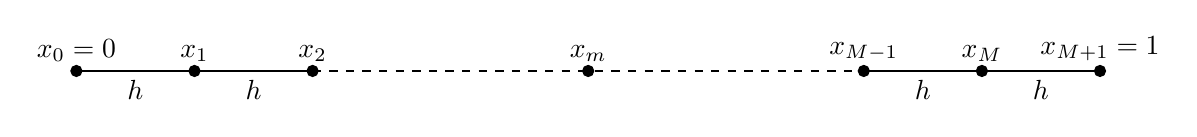
\begin{tikzpicture}
\draw (0,0) -- (3,0);
\draw[dashed] (3,0) -- (10,0);
\draw (10,0) -- (13,0);
\filldraw (0.0,0) circle (2pt) node[anchor=south] {$x_0 = 0$};
\filldraw (1.5,0) circle (2pt) node[anchor=south] {$x_1$};
\filldraw (3.0,0) circle (2pt) node[anchor=south] {$x_2$};
\filldraw (6.5,0) circle (2pt) node[anchor=south] {$x_m$};
\filldraw (10.0,0) circle (2pt) node[anchor=south] {$x_{M-1}$};
\filldraw (11.5,0) circle (2pt) node[anchor=south] {$x_{M}$};
\filldraw (13.0,0) circle (2pt) node[anchor=south] {$x_{M+1} = 1$};
\node[anchor=north] at (0.75, 0) {$h$};
\node[anchor=north] at (2.25, 0) {$h$};
\node[anchor=north] at (10.75, 0) {$h$};
\node[anchor=north] at (12.25, 0) {$h$};
\end{tikzpicture}
.
\end{center}
To generate finite difference methods of both first and second order, we approximate the second derivative at interior points using the forward difference and central difference
\begin{equation*}
\begin{aligned}
u_{xx}(x_m) & = \frac{u_m-2u_{m+1}+u_{m+2}}{h^2} + O(h^1) \qquad && (1 \leq m \leq M) \\
u_{xx}(x_m) & = \frac{u_{m-1}-2u_m+u_{m+1}}{h^2} + O(h^2) \qquad && (1 \leq m \leq M-1).
% TODO: how to use forward difference at point M-1 ???
\end{aligned}
\end{equation*}
To handle the Dirichlet boundary condition $u(0) = a$ at the left edge, we insert the trivial equation
\begin{equation*}
1 \cdot u_0 = a.
\end{equation*}
To handle the Neumann boundary condition $u_x(1) = b$ at the right edge to first or second order, we use
\begin{equation*}
\begin{aligned}
u_x(1) & = \frac{u_{M+1}-u_M}{h} & + & O(h^1) & = b\\
u_x(1) & = \frac{\frac{1}{2}u_{M-1}-2u_M+\frac{3}{2}u_{M+1}}{h} & + & O(h^2) & = b.
\end{aligned}
\end{equation*}
By writing all these equations in $(M+2) \times (M+2)$-matrix form $AU=b$, we obtain for example to second order
\begin{equation*}
\renewcommand{\arraystretch}{1.5} % stretch matrix vertically to make it square
\begin{bmatrix}
1 \\
+1/h^2 & -2/h^2 & +1/h^2 &   \\
  & \ddots & \ddots & \ddots & \\
  &   & +1/h^2 & -2/h^2 & +1/h^2 \\
  &   & +1/2h & -2/h & +3/2h \\
\end{bmatrix}
\begin{bmatrix}
U_0 \\ U_1 \\ \vdots \\ U_M \\ U_{M+1} \\
\end{bmatrix}
=
\begin{bmatrix}
a \\ f(x_1) \\ \vdots \\ f(x_M) \\ b \\
\end{bmatrix}
\end{equation*}

Some remarks:
\begin{itemize}
\item We could handle the Dirichlet boundary condition $u(0) = a$ differently by treating $U_0 = a$ as a known variable.
The system of equations is equivalent if we remove the first row and column of $A$ and the first entries in $U$ and $b$, but simultaneously modify the entry $f(x_1) \rightarrow f(x_1) - a/h^2$.
This approach is more consistent with treating $U_0$ as a known variable, since its precise value is defined by the Dirichlet boundary condition.
However, our approach of inserting a trivial equation $1 \cdot U_0 = a$ keeps the matrix dimensions independent of boundary conditions and makes it easier to reason with how the discretized differential operator represented by $A$ operates on the grid point $U_0$ in the same way it operates on all other grid points.
\item To handle different combinations of Dirichlet and Neumann boundary conditions at the ends, we simply replace the first or last rows of the matrix with the same type of equation.
Note that if the Neumann boundary condition is imposed at the left boundary, the last row of the matrix above would have to be both reversed and negated.
\item When Neumann boundary conditions are imposed at both ends, the solution is determined only up to a constant.
To see this for a general Poisson boundary value problem, note that if $u_{xx} = f(x)$, $u_x(0) = a$ and $u_x(1) = b$, then also $(u+C)_{xx} = f(x)$, $(u+C)_x(0) = a$ and $(u+C)_x(1) = b$ if $C$ is only a constant.
It can also be seen from the general solution for this particular source term that the constant $C_1$ is undetermined when the solution is subject to boundary conditions that involve derivatives only.
In this case, an additional constraint like $u(0) = 0$ must be imposed to define a unique solution.
\end{itemize}
With this in mind, it is now straightforward to solve the Poisson equation subject to any combination of Dirichlet and Neumann boundary conditions at the ends to both first and second order.

\begin{figure}
	\centering
	\begin{tikzpicture}
		\begin{groupplot}[
			group style={group size=2 by 3,horizontal sep=2cm,vertical sep=2cm},
			height=6cm,
			width=0.48\textwidth,
			]
			\nextgroupplot[title={$u(0)=0, \quad u_x(1)=1$},xmode=normal,ymode=normal,xlabel=$x$,ylabel=$u(x)$];
			\addplot [color=red] table [x=x,y=u] {exercise1/dir_neu.dat};
			\addplot [color=black, only marks, mark=x, each nth point=20] table [x=x,y=U] {exercise1/dir_neu.dat};
			\nextgroupplot[xmode=log,ymode=log,xlabel=$h$,ylabel=relative error];
			\addplot [color=red, mark=*] table [x=h,y=disc] {exercise1/dir_neu_err.dat};

			\nextgroupplot[title={$u(0)=1, \quad u(1)=1$},xmode=normal,ymode=normal,xlabel=$x$,ylabel=$u(x)$];
			\addplot [color=red] table [x=x,y=u] {exercise1/dir_dir.dat};
			\addplot [color=black, only marks, mark=x, each nth point=20] table [x=x,y=U] {exercise1/dir_dir.dat};
			\nextgroupplot[xmode=log,ymode=log,xlabel=$h$,ylabel=relative error];
			\addplot [color=red, mark=*] table [x=h,y=disc] {exercise1/dir_dir_err.dat};

			\nextgroupplot[title={$u_x(0)=0, \quad u_x(1)=1/2$},xmode=normal,ymode=normal,xlabel=$x$,ylabel=$u(x)$,scaled ticks=false, tick label style={/pgf/number format/fixed}];
			\addplot [color=red] table [x=x,y=u] {exercise1/neu_neu.dat};
			\addplot [color=black, only marks, mark=x, each nth point=20] table [x=x,y=U] {exercise1/neu_neu.dat};
			\nextgroupplot[xmode=log,ymode=log,xlabel=$h$,ylabel=relative error];
			\addplot [color=red, mark=*] table [x=h,y=disc] {exercise1/neu_neu_err.dat};
		\end{groupplot}
	\end{tikzpicture}
	\caption{\label{fig3}
		Analytical and numerical solutions (left) and convergence plots (right) for solutions to the Poisson equation subject to three different boundary conditions.
	}
\end{figure}

\iffalse
\begin{equation*}
\renewcommand{\arraystretch}{2.8} % stretch matrix vertically to make it square
\begin{bmatrix}
-2/h^2 & +1/h^2  & 0 & \cdots & 0 \\
+1/h^2  & -2/h^2 & +1/h^2  & \ddots & \vdots \\
0 & \ddots & \ddots & \ddots & 0 \\
\vdots & \ddots & +1/h^2 & -2/h^2 & +1/h^2\\
0 & \cdots & +1/2h & -2/h & +3/2h  \\
\end{bmatrix}
\begin{bmatrix}
U_1 \\ U_2 \\ \vdots \\ U_M \\ U_{M+1} \\
\end{bmatrix}
=
\begin{bmatrix}
f(x_1) - \alpha/h^2 \\ f(x_2) \\ \vdots \\ f(x_M) \\ \sigma \\
\end{bmatrix}
\end{equation*}






Note that when Neumann-Neumann boundary conditions are imposed, $C_1$ is undetermined and so the solution is determined only up to a constant.
To obtain a first order approximation of the second derivative at 





with the source term $f(x) = x + \cos(2 \pi x)$, subject to different kinds of boundary conditions
\begin{equation*}
\begin{aligned}
u(0) &= a, &\quad u(1) &= b &\qquad& \text{(Dirichlet-Dirichlet)} \\
u_x(0) &= a, &\quad u_x(1) &= b &\qquad& \text{(Neumann-Neumann)} \\
u(0) &= a, &\quad u_x(1) &= b &\qquad& \text{(Dirichlet-Neumann)}. \\
\end{aligned}
\end{equation*}


Inner points:
\begin{equation*}
\frac{U_{m+1} - 2 U_m + U_{m-1}}{h^2} = f(x_m)
\end{equation*}
Dirichlet, left:
\begin{equation*}
u(0) = U_0
\end{equation*}
Von-Neumann, left, 2nd order:
\begin{equation*}
u_x(0) \approx -\frac{(3/2)U_0 -2U_1 + (1/2)U_2}{h}
\end{equation*}
\fi


\begin{figure}
  \centering
  \begin{tikzpicture}
\begin{loglogaxis}[
  title=Error functions,
  xlabel={$M$},
  ylabel={$e_l$},
  legend pos=south west,
  ]

  \addplot table[y index=1] {exercise1/a_error.dat}
  coordinate [pos=0.24] (A)
  coordinate [pos=0.8] (B);
  \addplot table[y index=2] {exercise1/a_error.dat};
  \addplot table[y index=3] {exercise1/a_error.dat};

  \draw (A) -| (B)
  node [pos=0.25, anchor=south] {1}  %% Random value
  node [pos=0.75, anchor=west] {-1};

  \legend{$L_2$ discrete, $L_2$ continous step, $L_2$ continous interpolatino};
\end{loglogaxis}
\end{tikzpicture}

  \caption{Nice fig}
\end{figure}
